%
%%%%%%%%%%%%%%%%%%%%%%%%%%%%%%%%%%%%%%%%%%%%%%%%%%%
%
% E I N L E I T U N G
%
%%%%%%%%%%%%%%%%%%%%%%%%%%%%%%%%%%%%%%%%%%%%%%%%%%%
%
\chapter{Einleitung}
\label{cha:introduction}
%
%
Dieses Vorlagendokument soll das Erstellen der eigenen Bachelorarbeit mit LaTeX erleichtern. Es liefert ein bereits vollst�ndig konfiguriertes Dokument, in dem lediglich der Inhalt ausgetauscht werden muss. Formatierung sind voreingestellt und m�ssen nicht abge�ndert werden. Damit ist es m�glich, sich ohne gr��ere Einarbeitungszeit auf den Inhalt der Arbeit zu konzentrieren. \\
\\
\noindent \textbf{\textcolor{darkred}{Hinweis}}: Dies ist keine Anleitung, wie Sie eine Bachelorarbeit verfassen sollen und wie Sie dem wissenschaftlichen Anspruch des Inhalts gerecht werden. Diese Vorlage ist ein technisches Dokument und zeigt beispielsweise, wie Sie Fu�noten setzen und Literatur referenzieren. Nicht behandelt wird hier die Frage, wann und warum Sie eine Fu�note setzen oder eine Referenz verwenden.
%
%
%%%%%%%%%%%%%%%%%%%%%%%%%%%%%%%%%%%%%%%%%%%%%%%%%%%
%
% A U F B A U 
%
%%%%%%%%%%%%%%%%%%%%%%%%%%%%%%%%%%%%%%%%%%%%%%%%%%%
%
\section{Aufbau des Dokuments}
\label{sec:aufbau}
%
Diese Vorlage verwendet die \textit{memoir}-LaTeX-Klasse von Peter Wilson und erzeugt somit ein Buchdokument, das auch zweiseitig gedruckt werden sollte, da zwischen den Kapiteln Leerseiten erzeugt werden. Einstiegspunkt f�r die Bachelorarbeit ist die Datei \texttt{abschlussarbeit.tex}. Tragen Sie zun�chst den Titel der Arbeit und alle Namen ein. Bei hochschulinternen Bachlorarbeiten fallen die Eintragungen \textit{durchgef�hrt am} und \textit{Betreuer in der Firma} nat�rlich weg. \\

Neben den offensichtlichen Eintragungen f�r das Titelblatt wird in dieser Datei auch die Einteilung der Arbeit in Kapitel und Anh�nge vorgenommen. Verwenden Sie am besten f�r jedes Kapitel einen eigenen Unterordner. In jedem dieser Kapitelordner sollte ein Unterordner names \texttt{images} liegen. Dies erleichtert die Arbeit mit und die Suche nach den entsprechenden Abbildungen (siehe auch Abschnitt \ref{sec:abbildungen}). \\

Daneben werden in dieser Datei auch Zusatzpakete mit dem \texttt{usepackage}-Befehl eingebunden, Farben f�r eine farbliche Darstellung von Text und eventuelle Sonderzeichen wie beispielsweise das \textit{Copyright}-Zeichen \TCop oder das \textit{Trademark}-Zeichen \TTra definiert.
%
%
%%%%%%%%%%%%%%%%%%%%%%%%%%%%%%%%%%%%%%%%%%%%%%%%%%%
%
% Abbildungen
%
%%%%%%%%%%%%%%%%%%%%%%%%%%%%%%%%%%%%%%%%%%%%%%%%%%%
%
\section{Abbildungen}
\label{sec:abbildungen}
%
Bilder sollten im \texttt{.eps}-Format (Encapsulated PostScript) eingebunden werden. Wandeln Sie daher eine Grafik, die als \texttt{.jpg}, \texttt{.png} oder in einem anderen Dateiformat vorliegt, vor der Verwendung in Ihrer Bachelorarbeit entsprechend um. Alle g�ngigen Bildbearbeitungsprogramme wie beispielsweise Adobe Photoshop \footnote{http://www.adobe.com/de/products/photoshop/family/} oder Gimp \footnote{http://www.gimp.org/} sind in der Lage, Bilder ins \texttt{EPS}-Format zu exportieren.
%
\begin{figure}
  \centering
   {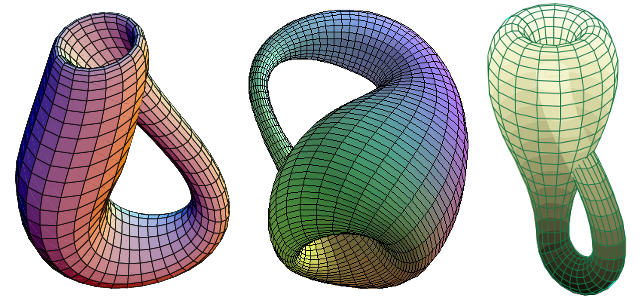
\epsfig{file = intro/images/klein_bottle.png, width=11.0cm}}
  \caption[Kleinsche Flasche]{Drei Versionen der Kleinschen Flasche. Die Objekte sind mit Mathematica (links, Quelle gemeinfrei), Maple (mitte, Quelle: T. Hall) und GnuPlot (rechts, Quelle: O. Alexandrov)	erstellt.}
  \label{fig:klein_bottle}
\end{figure}
%
Wenn Sie auf Abbildungen im Text verweisen wollen, verwenden Sie die \texttt{ref}-Marke: Die \textit{Kleinsche Flasche} \cite{schrijver89} (siehe Abbildung \ref{fig:klein_bottle}) ist ein geometrisches Objekt, das nur eine einzige Seite besitzt. Man kann also nicht zwischen \textit{innen} und \textit{au�en} unterscheiden. Beschriften Sie die Abbildungen ausf�hrlich. Verwenden Sie die beiden Textoptionen in der \texttt{caption}-Marke, um auch eine kurze Beschreibung f�r das Abbildungsverzeichnis zu erzeugen. \\
%
Vergessen Sie bitte nicht, die Eigent�mer eines Bildes zu nennen, wenn Sie ein Bild nicht selbst erstellt haben. \\
%
%
%%%%%%%%%%%%%%%%%%%%%%%%%%%%%%%%%%%%%%%%%%%%%%%%%%%
%
%  L I T E R A T U R V E R W E I S E
%
%%%%%%%%%%%%%%%%%%%%%%%%%%%%%%%%%%%%%%%%%%%%%%%%%%%
%
\section{Literaturverweise}
\label{sec:verweise}
%
Verweise auf Literatur, die Sie in der Ihrer Bachelorarbeit verwenden, sollten in der Datei \texttt{abschlussarbeit.bib} eingetragen werden. In dieser Datei k�nnen durchaus mehr Eintr�ge enthalten sein, als Sie in Ihrer Arbeit als Referenzen verwenden. LaTeX wird nur auch tats�chlich referenzierte Literatur in das Verzeichnis am Ende der Arbeit aufnehmen. Die freie Software LEd (siehe Kapitel \ref{cha:umgebung}) ist in der Lage, Vorlagen f�r die unterschiedlichsten Arten von Literatur aufzunehmen, wie beispielsweise B�cher, Artikel in Zeitschriften oder wissenschaftliche Ver�ffentlichungen in den \textit{Proceedings} von Konferenzen. Denken Sie bitte bei Ihrer Recherchearbeit daran, dass Sie von Rechnern der Hochschule aus freien Zugang zu einer Vielzahl von Online-Bibliotheken wie IEEE\footnote{http://ieeexplore.ieee.org/} und ACM\footnote{http://portal.acm.org/} haben.
%
%
%%%%%%%%%%%%%%%%%%%%%%%%%%%%%%%%%%%%%%%%%%%%%%%%%%%
%
%   F O R M E L N   U N D   T A B E L L E N
%
%%%%%%%%%%%%%%%%%%%%%%%%%%%%%%%%%%%%%%%%%%%%%%%%%%%
%
\section{Verwendung von Formeln und Tabellen}
\label{sec:formeln}
%
W�hrend Tabellen leider schnell un�bersichtlich werden k�nnen, spielt LaTeX bei Formeln sein volles Potential aus. Kein anderes Textsatzsystem erzeugt so schnell und einfach sch�ne Formeln. Im folgenden Abschnitt werden einige Textpassagen vorgestellt, die typische Formeln verwenden. Ein Blick an die entsprechenden Zeilen in der LaTeX-Datei zeigt Ihnen, wie diese Formeln entstehen.\\
\\
Formeln k�nnen direkt in den Text integriert werden: $x_i=x_{x-1} + x_{i-2}$ ist beispielsweise die Rechenvorschrift f�r die Fibonacci-Folge \cite{conway96}. \\
\\
``...Das Kameramodell basiert auf dem Prinzip der Lochkamera und wird f�r eine pr�zise Triangulierung um intrinsische Parameter wie etwa der Linsenverzeichnung erweitert: \\

\noindent \textbf{\textcolor{darkred}{Hinweis}}: Das $\Real$-Zeichen und die dunkelrote Textfarbe sind im Hauptdokument \texttt{abschlussarbeit.tex} definiert.
\begin{tabbing}
Platzhalter links \quad \= Platzhalter Mitte \quad \= Platzhalter rechts \kill
$T \in \Real^3$  \> der Brennpunkt und Ursprung des Kamerakoordinatensystems \\
                 \> im Weltkoordinatensystem und                             \\
$R \in SO_3$     \> die Rotation der Kamera im Weltkoordinatensystem
\end{tabbing}
Als intrinsische Parameter werden
\begin{tabbing}
Platzhalter links \quad \= Platzhalter Mitte \quad \= Platzhalter rechts \kill
$f \in \Real$             \> die Brennweite (fokale L�nge) der Kamera,                                          \\
$P=(u_0,v_0) \in \Real^2$ \> der Hauptpunkt des Bildes (engl.: \textit{principle point}), also der Schnittpunkt \\
                          \> der optischen Achse mit der dazu orthogonal stehenden Bildebene,                   \\
$r_u,r_v \in \Real$       \> Skalierungsfaktoren in x- und y-Richtung auf der Bildebene,                        \\
$s \in \Real$             \> ein Verzerrungsfaktor (engl.: \textit{skew}) der Kameralinse und                   \\
$\kappa \in \Real$        \> die radiale Verzeichnung der Kameralinse
\end{tabbing}
gew�hlt.\\
%
Mit Hilfe der Strahlens�tze ist die Projektion durch $(\nicefrac{-f \cdot x_c}{z_c}, \nicefrac{-f \cdot y_c}{z_c})^T$ zu berechnen. Die restlichen intrinsischen Kameraparameter lassen sich in der Kamerakalibrierungsmatrix $K$ mit
\begin{equation}
\label{eqn:K}
\left(\begin{array}{ccc}r_u&s&u_0\\0&r_v&v_0\\0&0&1 \end{array}\right) \cdot 
\left(\begin{array}{c}\nicefrac{-f \cdot x_c}{z_c}\\\nicefrac{-f \cdot y_c}{z_c}\\1\end{array}\right) = 
\underbrace{\left(\begin{array}{ccc}-f \cdot r_u&-f \cdot s&u_0\\0&-f \cdot r_v&v_0\\0&0&1 \end{array}\right)}_{=K} \cdot 
\left(\begin{array}{c}\nicefrac{x_c}{z_c}\\\nicefrac{y_c}{z_c}\\1\end{array}\right)
\end{equation}
zusammenfassen. Diese Matrix wird so genannt, da alle intrinsischen Konstanten der Kalibrierung in einer einzigen Matrix enthalten sind. \\
%
Die Summe der $m$ Abst�nde zwischen Originalpunkt und projiziertem Punkt in der Bildebene der zweiten Kamera wird mit
\begin{equation}
\sum_{i=1..m}r_i = \sum_{i=1..m} \Vert\tilde U^2_i - U^2_i \Vert
\end{equation}
minimiert.''\\
%

Nun ein Beispiel, bei dem zwei Formeln in einer Zeile stehen, das verbindende \textit{UND} aber nicht als Formeltext, sondern als normaler Flusstext erscheint: ``...Als erster Schritt der Rekonstruktion werden beide 2D-Punkte um einen Tiefenwert erweitert, um 3D-Koordinaten zu erhalten:''
%
\begin{equation}
\bar{U}^1=\left(\begin{array}{c}U^1\\-f_1\end{array}\right) \in \Real^3 \quad \mbox{und} \quad
\bar{U}^2=\left(\begin{array}{c}U^2\\-f_2\end{array}\right) \in \Real^3
\end{equation}
%

Am Ende dieses Abschnitts noch ein Beispiel f�r eine Tabelle:\\
``Die folgende Tabelle \ref{tab:vergleich} stellt die vier Verfahren in einem direkten Vergleich in Bezug auf die drei Parameter gegen�ber:''
%
%
%  T A B L E   V E R G L E I C H
%
\begin{table}[H]
\centering{
\caption{Vergleich verschiedener Algorithmen.}
\label{tab:vergleich}
\begin{tabular}{p{2.5cm}p{2.5cm}p{2.5cm}p{2.5cm}p{2.5cm}}
  \hline \addlinespace
   & \textbf{Verfahren 1} & \textbf{Verfahren 2} & \textbf{Verfahren 3} & \textbf{Verfahren 4} \\
  \addlinespace \hline \addlinespace
  \textbf{Lexikoneintrag} & nein & ja & ja & nein \\
  \addlinespace \hline \addlinespace
  \textbf{Trainings\-aufwand} & keiner & keiner & 2 min bei \newline Optimierung\textsuperscript{1} & keiner \\
  \addlinespace \hline \addlinespace
  \textbf{Ergebnis} & 22 sec & 32 sec & 30 sec & 13 sec \\
  \addlinespace \hline
\end{tabular}}
\end{table}
%\vspace{1mm}
\noindent \textsuperscript{1} Anmerkungen zu Tabelleneintr�gen k�nnen am Ende der Tabelle erkl�rt werden. \vspace{2mm} \\
%
Lorem ipsum dolor sit amet, consectetur adipisici elit, sed eiusmod tempor incidunt ut labore et dolore magna aliqua. Ut enim ad minim veniam, quis nostrud exercitation ullamco laboris nisi ut aliquid ex ea commodi consequat. Quis aute iure reprehenderit in voluptate velit esse cillum dolore eu fugiat nulla pariatur. Excepteur sint obcaecat cupiditat non proident, sunt in culpa qui officia deserunt mollit anim id est laborum. \\
